% ============================================================
%  书末习题（原书印刷页 561–570；PDF 页 = 印刷页 + 20）
%  底本：高等教育出版社《固体理论》第二版
%  体例（已逐页核对原书 p581–p590）：原书习题区**不按章分组**，
%    十二章的习题自 1. 至 50. 连续编号排版，无"第一章…"组头，
%    故本文件不设组头（任务单所拟"按章分组、组内另起 1."与原书
%    版面不符，以原书为准）；习题内公式一律不编号；题内带编号
%    条目"(1)"照录，纯公式条目用 equation* 左侧缀"(n)"。
%
%  已修正的 OCR 错误（除全角句点转"."、删 ~、收紧 \mathrm{d}、
%  拆开与中文粘连的行内公式等常规项外，均对照 p581–p590 页面）：
%  1. 题1  k=Σ_j(n_j/N_j)b_j 分子上衍出的点状杂符已删（p581）。
%  2. 题3  OCR"Ω^α=(2π)³"按 p581 复原为 ΩΩ*=(2π)³。
%  3. 题4  ψ_{n,k+K} 尾部衍出的杂符";"已删（p581）。
%  4. 题6  ω 的误置粗体已去；a⁺ 按 p581 复原（OCR \textbf 乱码）。
%  5. 题7  ω_σ(k) 的 OCR 杂符 \stackrel{,}{(} 复原为 (k)（p581）。
%  6. 题8  极化矢量 OCR \ell_{kσ} 按原书复原为 e_{kσ}（p582）；
%      弹性波方程分量上标 u^{x,y,z} 照原书排。
%  7. 题9  OCR"ω_L = ε₀−ε_∞"语序错乱，按 p582 复原为"ω_L 与 ω_T
%      为纵、横波频率"；4πγ₁₂² 下标结构复原。
%  8. 题11 OCR c_m(T) 按原书复原为 C_m(T)（大写 C、正体下标，p582）。
%  9. 题12 ℋ_{u'}、J_{u'} 按原书复原为 ℋ_{ll'}、J_{ll'}；(2) 中第二
%      列矢 (0 1)_{l'} 按 p582 复原。
% 10. 题13 Ŝ^γŜ_{l'}^γ → Ŝ_l^yŜ_{l'}^y；cos[k*(l−l')] →
%      cos[k·(l−l')]；求和下标 ι → l（p582）。
% 11. 题14 晶场 OCR ±B_{A^±} 复原为 ±B_A；ħω_k^x → ħω_k^±（p582–583）。
% 12. 题16 "(h=1)"按原书复原为 (ħ=1)（两处，p583）。
% 13. 题18 ω₁ 项 b_{−k}⁺b_k⁺ 顺序照原书（OCR 衍空格清理，p583）。
% 14. 题19 (1) OCR"[[H,ρq],ρ−q] = − m"按 p583 复原为 −(Nq²/m)；
%      "严格本征值"OCR 乱码（→^j 格）复原。
% 15. 题21 ε^{RPA}(q,ω) 两处 OCR 乱码按 p584 重排；ℒ(q) 定义式
%      OCR"="复原为"≡"。
% 16. 题24 (2)"T→0 K"OCR 缺箭头已补（p584）。
% 17. 题26 关联函数两行式 OCR 严重乱码，按 p585 重排复原
%      （g_{↑↑}、F(r) 及 j₁ 球贝塞耳函数）。
% 18. 题27 散射矩阵元 cases 块（−V 能壳内/0 能壳外）按 p585 复原；
%      Δ(K) 分母 exp[2/(g(k_F,K)V)]−1 补回 V；g(k_F,K) 乱码复原。
% 19. 题28 提示语 OCR 缺左方括号，按 p585 补"［提示：…］"。
% 20. 题29 g_s(ξ)/g_n(0) 两行 cases OCR 乱码按 p585 复原。
% 21. 题31 tanh(½β£_k) 的 £ 按原书复原为 ξ（p586）。
% 22. 题32 条件"T ≪ T_c ≪ T_c"OCR 重衍 → T ≪ T_c；
%      H_c(0)=ΔΛ(0)√(4πg(0)) → H_c(0)=Δ(0)√(4πg(0))（p586）。
% 23. 题33 ⟨H̄_int(λ)⟩ 下标 OCR 误作 τ → T；G(λ) 定义式乱码按
%      p586 复原。
% 24. 题34 高温区条件 (T_c−T<T_c) 按原书复原为 (T_c−T≪T_c)（p586）。
% 25. 题37 指数因子 (n−1)²P²/ħ² 原书排印 n/η 混用，按题内定义的 η
%      统一为 (η−1)²P²/ħ²（p566–567）；"而 r 的坐标原点取在电子上"
%      OCR 漏 r 已补。
% 26. 题38 e^{-s}He^s → e^{−S}He^{S}（母函数 S 大写，p567）。
% 27. 题39 对角形式两行式 OCR 乱码按 p567 复原。
% 28. 题40 Σ_r(ω) 定义 OCR"\sum_{±}"→ Σ_k（p567）。
% 29. 题41 E_k=−Wcos k 的条件 OCR"∧π<−W⩽E_k⩽W"乱码按 p567 复原为
%      "或 −W⩽E_k⩽W"；(2) 谱函数 A(ω) 中的 δ 函数 OCR 误作
%      \hat{ω}，按 p568 复原；Ẽ_d 式中 √(W⁴+4B²) 乱码复原（p568）。
% 30. 题44 C⁺_{kd} → C⁺_{kσ}；"严格解"OCR 乱码（→^± 格）复原（p568）。
% 31. 题45 ρ_f 式 (1/2D)·V²/(ω−E_f)² 的分母平方 OCR 衍落，已归位（p569）。
% 32. 题46 自洽方程被积式 OCR"(σ−1/π)Im…"按 p569 复原为
%      (−1/π)Im G_cf(ω+iη)。
% 33. 题47 (2)"\dot{T}=0 K"→ T=0 K；√(Γ̃²+(E_f−μ)²) 式按 p570 复原。
% 34. 题48 无双占条件 OCR"n_i≠n_i≠"按 p570 复原为 n_{i↑}n_{i↓}=0；
%      n_{iσ̄}（σ 带横杠，两处）复原。
% 35. 题49 μ_B 下标 OCR 误作 8 → B；m≡⟨n_↑⟩−⟨n_↓⟩ 乱码复原（p570）。
%
%  遗留问题：
%  · 习题图 1（题7，原书 p581 右下）为占位图 figures/figx-1.pdf，
%    待重绘代理绘制（六角形简约区BZ，含 Γ、T、Σ、M、K 及直角标记）。
%  · 题36"当 γ≪1 时上式简化为式(9.2.9)"照原书排（p566）；按物理
%    推断疑为"γ≫k"之误，未改。
%  · 题46 n_t 下标照原书（与 ch11 的 n_t=每格点总电子数一致，未改）。
% ============================================================
\chapter*{习题}
\markboth{习题}{}
\addcontentsline{toc}{chapter}{习题}

{\heiti 1.} 设 $\boldsymbol{k}$ 与 $\boldsymbol{k}'$ 均为BZ中波矢，$\boldsymbol{l}=\sum_{i}l_{i}\boldsymbol{a}_{i}$，$\boldsymbol{k}=\sum_{j}\frac{n_{j}}{N_{j}}\boldsymbol{b}_{j}$，$N_{1}N_{2}N_{3}=N$.试直接证明下列正交关系
\begin{equation*}
\begin{aligned}
  &\text{(1)}\ \ N^{-1}\sum_{l}\mathrm{e}^{\pm\mathrm{i}(\boldsymbol{k}-\boldsymbol{k}')\cdot\boldsymbol{l}}=\delta_{\boldsymbol{k}\boldsymbol{k}'}\\
  &\text{(2)}\ \ N^{-1}\sum_{k\in\mathrm{BZ}}\mathrm{e}^{\pm\mathrm{i}\boldsymbol{k}\cdot(\boldsymbol{l}-\boldsymbol{l}')}=\delta_{\boldsymbol{l}\boldsymbol{l}'}
\end{aligned}
\end{equation*}

{\heiti 2.} 设 $f(\boldsymbol{r})$ 为正点阵的周期函数，证明当 $\boldsymbol{k}$ 不等于倒格矢 $\boldsymbol{K}$ 时
\begin{equation*}
  \int f(\boldsymbol{r})\,\mathrm{e}^{\mathrm{i}\boldsymbol{k}\cdot\boldsymbol{r}}\,\mathrm{d}\boldsymbol{r}=0
\end{equation*}

{\heiti 3.} 证明 $\Omega\Omega^{*}=(2\pi)^{3}$

{\heiti 4.} 试用平面波法论证布洛赫函数
\begin{equation*}
  \psi_{n,\boldsymbol{k}}(\boldsymbol{r})=\psi_{n,\boldsymbol{k}+\boldsymbol{K}}(\boldsymbol{r})
\end{equation*}
其中 $\boldsymbol{k}$ 为简约波矢，$\boldsymbol{K}$ 为倒格矢，$n$ 为带指标.

{\heiti 5.} 设晶格周期场 $V=0$，试应用布洛赫定理求简约区（BZ）中单电子的能量和状态波函数，并作出能带曲线的一维示意图.

{\heiti 6.} 讨论在均匀外电场 $\mathcal{E}$ 中质量为 $M$，带电量为 $e$ 和频率为 $\omega$ 的一维谐振子系统.试证用玻色算子 $a$ 与 $a^{+}$ 表示的哈密顿量为
\begin{equation*}
  H=\hbar\omega\Bigl(a^{+}a+\frac{1}{2}\Bigr)+\lambda\left(a+a^{+}\right)
\end{equation*}
其中 $\lambda=e\mathcal{E}\sqrt{\dfrac{\hbar}{2M\omega}}$.

{\heiti 7.} 讨论二维密排六角晶格的格波特性.设 $a$ 为晶格常数，$f$ 代表最近邻原子间的线弹性力常数，其简约区BZ如下图所示，求BZ中 $\Sigma$ 线（包括 $\Gamma$，$M$ 点）和 $T$ 线（包括 $\Gamma$，$K$ 点）上的：

(1) 动力矩阵 $D_{\alpha\beta}(\boldsymbol{k})=?$

(2) 格波频率 $\omega_{\sigma}(\boldsymbol{k})$ 和极化矢量 $\boldsymbol{e}_{k\sigma}=?$

\par\nopagebreak\noindent\begin{minipage}{\linewidth}\centering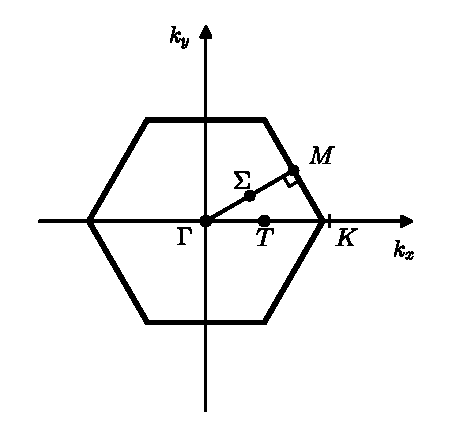
\includegraphics[width=4.5cm]{figx-1.pdf}\\[0.3em]{\small 习题图 1}\end{minipage}\par\nopagebreak

{\heiti 8.} 设立方晶体的弹性波方程为
\begin{equation*}
\begin{aligned}
  \rho\frac{\partial^{2}u^{x}}{\partial t^{2}}
  ={}&C_{11}\frac{\partial^{2}}{\partial x^{2}}u^{x}
  +C_{44}\Bigl(\frac{\partial^{2}}{\partial y^{2}}+\frac{\partial^{2}}{\partial z^{2}}\Bigr)u^{x}\\
  &+(C_{12}+C_{44})\frac{\partial}{\partial x}\Bigl(\frac{\partial u^{y}}{\partial y}+\frac{\partial u^{z}}{\partial z}\Bigr)
\end{aligned}
\end{equation*}
\begin{equation*}
\begin{aligned}
  \rho\frac{\partial^{2}u^{y}}{\partial t^{2}}
  ={}&C_{11}\frac{\partial^{2}}{\partial y^{2}}u^{y}
  +C_{44}\Bigl(\frac{\partial^{2}}{\partial z^{2}}+\frac{\partial^{2}}{\partial x^{2}}\Bigr)u^{y}\\
  &+(C_{12}+C_{44})\frac{\partial}{\partial y}\Bigl(\frac{\partial u^{z}}{\partial z}+\frac{\partial u^{x}}{\partial x}\Bigr)
\end{aligned}
\end{equation*}
\begin{equation*}
\begin{aligned}
  \rho\frac{\partial^{2}u^{z}}{\partial t^{2}}
  ={}&C_{11}\frac{\partial^{2}}{\partial z^{2}}u^{z}
  +C_{44}\Bigl(\frac{\partial^{2}}{\partial x^{2}}+\frac{\partial^{2}}{\partial y^{2}}\Bigr)u^{z}\\
  &+(C_{12}+C_{44})\frac{\partial}{\partial z}\Bigl(\frac{\partial u^{x}}{\partial x}+\frac{\partial u^{y}}{\partial y}\Bigr)
\end{aligned}
\end{equation*}
其中 $C_{ij}$ 为弹性常数，求沿 $[111]$ 方向的格波频率 $\omega_{\sigma}(\boldsymbol{k})$ 和极化矢量 $\boldsymbol{e}_{k\sigma}$.

{\heiti 9.} 设长波纵光学模的哈密顿密度为
\begin{equation*}
  \mathscr{H}_{0}=\frac{1}{2}\dot{\boldsymbol{W}}_{\mathrm{L}}^{2}
  +\frac{1}{2}\omega_{\mathrm{T}}^{2}\boldsymbol{W}_{\mathrm{L}}^{2}
  -\gamma_{12}\boldsymbol{W}_{\mathrm{L}}\cdot\boldsymbol{E}_{\mathrm{L}}
  -\frac{1}{2}\gamma_{22}\boldsymbol{E}_{\mathrm{L}}^{2}
\end{equation*}
其中 $E_{\mathrm{L}}=-\dfrac{4\pi\gamma_{12}}{1+4\pi\gamma_{22}}W_{\mathrm{L}}$，$1+4\pi\gamma_{22}=\varepsilon_{\infty}$，$4\pi\gamma_{12}^{2}=(\varepsilon_{0}-\varepsilon_{\infty})\omega_{\mathrm{T}}^{2}$，$\omega_{\mathrm{L}}$ 与 $\omega_{\mathrm{T}}$ 为纵、横波频率.试将系统的哈密顿量 $H_{0}=\int\mathscr{H}_{0}\,\mathrm{d}r$ 写成标准二次量子化形式.

{\heiti 10.} 利用色散关系式(2.2.30)计算一维双原子链的声子态密度，并作出声子频谱的示意图.

{\heiti 11.} 求立方晶格（sc、bcc、fcc）铁磁体中磁振子（magnons）的低温比热容 $C_{\mathrm{m}}(T)$.

{\heiti 12.} 讨论 $S=\frac{1}{2}$ 的两个自旋系统，设其哈密顿量为
\begin{equation*}
  \mathcal{H}_{ll'}=-2J_{ll'}\hat{\boldsymbol{S}}_{l}\cdot\hat{\boldsymbol{S}}_{l'}
\end{equation*}
试证明：

(1) $|\uparrow,\uparrow\rangle\equiv\binom{1}{0}_{\! l}\binom{1}{0}_{\! l'}$ 是 $\mathcal{H}_{ll'}$ 的本征态；

(2) $|\uparrow,\downarrow\rangle\equiv\binom{1}{0}_{\! l}\binom{0}{1}_{\! l'}$ 不是 $\mathcal{H}_{ll'}$ 的本征态.

{\heiti 13.} 若用
\begin{equation*}
  |k\rangle=\frac{1}{\sqrt{2SN}}\sum_{l}\mathrm{e}^{\mathrm{i}\boldsymbol{k}\cdot\boldsymbol{l}}\hat{S}_{l}^{-}|0\rangle
\end{equation*}
描述铁磁自旋晶格系统的最低激发态，试严格证明
\begin{equation*}
  \langle k|\bigl(\hat{S}_{l}^{x}\hat{S}_{l'}^{x}+\hat{S}_{l}^{y}\hat{S}_{l'}^{y}\bigr)|k\rangle
  =\frac{2S}{N}\cos\bigl[\boldsymbol{k}\cdot(\boldsymbol{l}-\boldsymbol{l}')\bigr]
\end{equation*}
并求系统的元激发能量 $\hbar\omega_{k}$，其中 $N$ 为格点数，$S$ 为格点上的自旋值，而 $|0\rangle$ 为铁磁基态.

{\heiti 14.} 证明在外磁场 $\boldsymbol{B}=\boldsymbol{B}\boldsymbol{z}$ 和各向异性晶场 $\pm\boldsymbol{B}_{A}$ 中（其中a子格取“+”号，b子格取“−”号）反铁磁体的自旋波量子为
\begin{equation*}
  \hbar\omega_{k}^{\pm}=2Z|J|S\sqrt{\Bigl(1+\frac{g\mu_{\mathrm{B}}B_{A}}{2Z|J|S}\Bigr)^{2}-\gamma_{k}^{2}}\pm g\mu_{\mathrm{B}}B
\end{equation*}
这里 $\gamma_{k}\equiv\frac{1}{2}\sum_{\boldsymbol{\delta}}^{\prime}\mathrm{e}^{-\mathrm{i}\boldsymbol{k}\cdot\boldsymbol{\delta}}$.

{\heiti 15.} 试用 $u-v$ 变换方法求
\begin{equation*}
  H=E_{0}a^{+}a+E_{1}\left(a^{+}a^{+}+aa\right)
\end{equation*}
的元激发严格解，其中 $a$ 与 $a^{+}$ 为玻色算子，$E_{0}$ 与 $E_{1}$ 为常数，且 $E_{0}>2E_{1}$.

{\heiti 16.} 设磁振子与声子互作用系统的哈密顿量为
\begin{equation*}
  H=\sum_{k}\bigl\{\bigl(\omega_{k}^{\mathrm{m}}a^{+}_{k}a_{k}
  +\omega_{k}^{\mathrm{p}}b^{+}_{k}b_{k}\bigr)
  +V_{k}\left(a_{k}b^{+}_{k}+a^{+}_{k}b_{k}\right)\bigr\}
\end{equation*}
其中 $\omega_{k}^{\mathrm{m}}$ 为磁振子能量（$\hbar=1$），$\omega_{k}^{\mathrm{p}}$ 为声子能量（$\hbar=1$），$a_{k}$ 为磁振子算符，$b_{k}$ 为声子算符，$V_{k}$ 为耦合系数，试求

(1) 使 $H$ 对角化的变换（变换形式及对角化条件）；

(2) 当 $\omega_{k}^{\mathrm{m}}=\omega_{k}^{\mathrm{p}}=\omega_{k}$ 时，互作用系统的元激发能量.

{\heiti 17.} 已知含 $N$ 个元胞复式晶格的电子TBA哈密顿量为
\begin{equation*}
  H=E_{1}\sum_{i}a^{+}_{i}a_{i}+E_{2}\sum_{j}b^{+}_{j}b_{j}
  +W\sum_{i}\sum_{\boldsymbol{\delta}}^{\prime}
  \left(a^{+}_{i}b_{i+\boldsymbol{\delta}}+b^{+}_{i}a_{i+\boldsymbol{\delta}}\right)
\end{equation*}
其中 $a_{i}$ 与 $b_{j}$ 是元胞中A、B原子周围的局域电子算符，晶格配位数设为 $Z$.试将 $H$ 对角化，并求出能带电子的能量.

{\heiti 18.} 设超流玻色系统的哈密顿量近似为
\begin{equation*}
  H=\sum_{k}^{\prime}\bigl\{\omega_{0}\bigl(b^{+}_{k}b_{k}+b^{+}_{-k}b_{-k}\bigr)
  +\omega_{1}\bigl(b_{k}b_{-k}+b^{+}_{-k}b^{+}_{k}\bigr)\bigr\}
\end{equation*}
其中 $\omega_{0}=\varepsilon_{k}+NV_{k}$，$\omega_{1}=NV_{k}$，$\varepsilon_{k}=\frac{k^{2}}{2M}$，$V_{k}>0$，$\sum_{k}^{\prime}(\cdots)$ 表示求和时 $k\neq0$.试将 $H$ 对角化，求出其元激发能量（取 $\hbar=1$ 单位），并讨论元激发谱中是否存在能隙？

{\heiti 19.} 证明互作用电子系统当取 $\hbar=1$ 时有下列严格关系：
\begin{equation*}
\begin{aligned}
  &\text{(1)}\ \ \bigl[\bigl[H,\rho_{\boldsymbol{q}}\bigr],\rho_{-\boldsymbol{q}}\bigr]
  =-\Bigl(\frac{Nq^{2}}{m}\Bigr);\\
  &\text{(2)}\ \ \sum_{n}\omega_{n0}\bigl\{\bigl|\langle n|\rho_{\boldsymbol{q}}|0\rangle\bigr|^{2}
  +\bigl|\langle n|\rho_{-\boldsymbol{q}}|0\rangle\bigr|^{2}\bigr\}=\frac{Nq^{2}}{m};\\
  &\text{(3)}\ \ \int_{0}^{\infty}\mathrm{d}\omega\,\omega\,
  \mathrm{Im}\Bigl[\frac{1}{\varepsilon(\boldsymbol{q},\omega)}\Bigr]
  =-\Bigl(\frac{\pi\omega_{\mathrm{p}}^{2}}{2}\Bigr),
\end{aligned}
\end{equation*}
其中 $\omega_{\mathrm{p}}^{2}=\frac{4\pi Ne^{2}}{m}$，$\rho_{\boldsymbol{q}}=\sum_{k}C^{+}_{k}C_{k+\boldsymbol{q}}$，$\omega_{n0}=\mathcal{E}_{n}-\mathcal{E}_{0}$，$\mathcal{E}_{n}$ 为 $H$ 的严格本征值.

{\heiti 20.} 利用附录B中的严格介电函数公式(B.1)，证明关系式
\begin{equation*}
  \lim_{\omega\to\infty}\mathrm{Re}\Bigl[\frac{1}{\varepsilon(\boldsymbol{q},\omega)}\Bigr]=1+\frac{\omega_{\mathrm{p}}^{2}}{\omega^{2}}
\end{equation*}

{\heiti 21.} 试用格林函数方法证明

(1) 哈特利-福克近似的介电函数
\begin{equation*}
  \frac{1}{\varepsilon^{\mathrm{HFA}}(\boldsymbol{q},\omega)}=1-\mathcal{L}(q)
\end{equation*}

(2) 无规相近似的介电函数
\begin{equation*}
  \varepsilon^{\mathrm{RPA}}(\boldsymbol{q},\omega)=1+\mathcal{L}(q)
\end{equation*}
其中
\begin{equation*}
  \mathcal{L}(q)\equiv\frac{v(q)}{\hbar}\sum_{k}n_{k}
  \Bigl\{\frac{1}{\omega_{kq}-(\omega+\mathrm{i}\eta)}
  +\frac{1}{\omega_{kq}+(\omega+\mathrm{i}\eta)}\Bigr\}
\end{equation*}
这里 $\eta=+0$.

{\heiti 22.} 证明三维电子气的等离激元的长波色散曲线为
\begin{equation*}
  \omega_{q}=\sqrt{\omega_{\mathrm{p}}^{2}+\frac{3}{5}q^{2}v_{\mathrm{F}}^{2}}
\end{equation*}
其中 $v_{\mathrm{F}}=\frac{\hbar k_{\mathrm{F}}}{m}$，$\omega_{\mathrm{p}}^{2}=\frac{4\pi Ne^{2}}{m}$.

{\heiti 23.} 求一维电子气 $q<2k_{\mathrm{F}}$ 时个别激发的下限 $\omega_{kq}^{\min}$，并在 $\omega-q$ 图上作出其曲线.

{\heiti 24.} 用介电函数讨论快速电子激发金属中等离激元的能量损失问题.设有一个速度为 $v$ 的快速电子注入金属.

(1) 证明此电子每秒的能量损耗为
\begin{equation*}
  -\Bigl(\frac{e}{\pi}\Bigr)^{2}\int\frac{\mathrm{d}^{2}q}{q^{2}}\int_{0}^{\infty}\mathrm{d}\omega\,\omega\,
  \mathrm{Im}\Bigl[\frac{1}{\varepsilon(\boldsymbol{q},\omega)}\Bigr]\delta(\omega-\boldsymbol{q}\cdot\boldsymbol{v})
\end{equation*}

(2) 试用无规相近似结果证明，当 $T\to0$ K 时在等离子集体振荡区（长波、高频限）
\begin{equation*}
  -\mathrm{Im}\Bigl[\frac{1}{\varepsilon^{\mathrm{RPA}}(q,\omega)}\Bigr]\approx\frac{\pi}{2}\omega_{\mathrm{p}}\delta(\omega-\omega_{\mathrm{p}})
\end{equation*}

{\heiti 25.} 试计算 $T>0$ K 时离子晶体中极化子的寿命 $\tau$.证明当 $k\ll\gamma\equiv(2m\omega_{\mathrm{L}}/\hbar)^{1/2}$ 时极化子在有限温度的
\begin{equation*}
  \frac{1}{\tau}\approx\frac{2\alpha\omega_{\mathrm{L}}}{\mathrm{e}^{\beta\hbar\omega_{\mathrm{L}}}-1}
\end{equation*}
讨论此结果的物理意义，其中 $\alpha$ 为极化子的耦合常数.

{\heiti 26.} 用哈特利-福克近似证明，在 $N$ 个电子系统中自旋平行电子对的关联函数
\begin{equation*}
\begin{aligned}
  &g_{\uparrow\uparrow}(\boldsymbol{r})=\frac{1}{N(N-1)}\sum_{i,j}
  \bigl|\phi_{\uparrow\uparrow}(\boldsymbol{r}_{i},\boldsymbol{r}_{j})\bigr|^{2}
  =\frac{1}{2}\bigl\{1-F^{2}(\boldsymbol{r})\bigr\}\\
  &F(\boldsymbol{r})=\frac{3}{k_{\mathrm{F}}r}\,j_{1}(k_{\mathrm{F}}r)
  =\frac{3}{(k_{\mathrm{F}}r)^{3}}\bigl[\sin(k_{\mathrm{F}}r)-(k_{\mathrm{F}}r)\cos(k_{\mathrm{F}}r)\bigr]
\end{aligned}
\end{equation*}
其中 $\boldsymbol{r}=\boldsymbol{r}_{i}-\boldsymbol{r}_{j}$、$\phi_{\uparrow\uparrow}(\boldsymbol{r}_{i},\boldsymbol{r}_{j})$ 代表自旋平行电子对哈特利-福克近似波函数的空间部分.

{\heiti 27.} 设总波矢为 $\boldsymbol{K}=\boldsymbol{k}_{1}+\boldsymbol{k}_{2}$ 的一对自旋反平行电子间的互作用势能为 $V(\boldsymbol{r})$，其散射矩阵元可近似写成
\begin{equation*}
\begin{aligned}
  V_{kk'}&=\frac{1}{N\Omega}\int V(\boldsymbol{r})\,
  \mathrm{e}^{\mathrm{i}(\boldsymbol{k}-\boldsymbol{k}')\cdot\boldsymbol{r}}\,\mathrm{d}\boldsymbol{r}\\
  &=\begin{cases}
    -V & \left(E_{\mathrm{F}}<E_{k}<E_{\mathrm{F}}+\hbar\omega_{\mathrm{D}}\text{，能壳内}\right)\\
    0 & \left(\text{能壳外}\right)
  \end{cases}
\end{aligned}
\end{equation*}
试证明电子对的能量
\begin{equation*}
  E=\frac{\hbar^{2}K^{2}}{4m}+\frac{\hbar^{2}k_{\mathrm{F}}^{2}}{m}-\Delta(\boldsymbol{K})
\end{equation*}
其中
\begin{equation*}
  \Delta(\boldsymbol{K})=\frac{2\hbar\omega_{\mathrm{D}}}{\exp\Bigl[\dfrac{2}{g(k_{\mathrm{F}},\boldsymbol{K})V}\Bigr]-1}
\end{equation*}
这里 $g(k_{\mathrm{F}},\boldsymbol{K})$ 代表费密面上总波矢为 $\boldsymbol{K}$ 的电子态密度.

{\heiti 28.} 证明库柏对的均方根半径
\begin{equation*}
  \sqrt{\langle r^{2}\rangle}\approx\frac{2}{\sqrt{3}}\,\frac{\hbar v_{\mathrm{F}}}{E}
\end{equation*}
［提示：库柏对是 $\boldsymbol{K}=0$ 的 $\uparrow$，$\downarrow$ 自旋电子对］

{\heiti 29.} 证明BCS超导体中准粒子的态密度 $g_{\mathrm{s}}(\xi)$ 与费密面上正常相态密度 $g_{\mathrm{n}}(0)$ 之比为
\begin{equation*}
  \frac{g_{\mathrm{s}}(\xi)}{g_{\mathrm{n}}(0)}=
  \begin{cases}
    \dfrac{\xi}{\sqrt{\xi^{2}-\Delta^{2}}} & \left(\left|\xi\right|>\Delta\right)\\[0.8em]
    0 & \left(\left|\xi\right|<\Delta\right)
  \end{cases}
\end{equation*}
其中 $\xi=\sqrt{\varepsilon^{2}+\Delta^{2}}$，$\varepsilon$ 为从费密面算起的自由电子能量.

{\heiti 30.} 试证明BCS超导体中总粒子数的涨落为
\begin{equation*}
  \frac{\langle\hat{N}^{2}\rangle-\langle\hat{N}\rangle^{2}}{\langle\hat{N}\rangle^{2}}
  =\frac{\displaystyle\sum_{k}\left(u_{k}v_{k}\right)^{2}}{\Bigl(\displaystyle\sum_{k}v_{k}^{2}\Bigr)^{2}}
\end{equation*}
其中 $\hat{N}=\sum_{k}\left(C^{+}_{k}C_{k}+C^{+}_{-k}C_{-k}\right)$，$\langle\cdots\rangle$ 代表对BCS基态的平均.

{\heiti 31.} 用BCS理论证明 $T>0$ K 时超导体中的平均占据数
\begin{equation*}
  \langle C^{+}_{k}C_{k}\rangle_{T}=\frac{1}{2}\Bigl[1-\bigl(\varepsilon_{k}/\xi_{k}\bigr)\tanh\Bigl(\frac{1}{2}\beta\xi_{k}\Bigr)\Bigr]
\end{equation*}

{\heiti 32.} 试用BCS理论证明超导体的临界磁场在 $T\ll T_{\mathrm{c}}$ 时为
\begin{equation*}
  H_{\mathrm{c}}(T)=H_{\mathrm{c}}(0)\Bigl(1-\frac{\mathrm{e}^{2\gamma}}{3}\,\frac{T^{2}}{T_{\mathrm{c}}^{2}}\Bigr)
\end{equation*}
其中 $H_{\mathrm{c}}(0)=\Delta(0)\sqrt{4\pi g(0)}$，$\gamma=0.5772$.

{\heiti 33.} 利用 $\overline{H}(\lambda)=\overline{H}_{0}+\overline{H}_{\mathrm{int}}(\lambda)$，$\overline{H}_{0}=H_{0}-\mu N$ 和 $\overline{H}_{\mathrm{int}}(\lambda)=\lambda\overline{H}_{\mathrm{int}}$ 以及吉布斯自由能 $G(\lambda)=-k_{\mathrm{B}}T\ln\mathrm{Tr}\left(\mathrm{e}^{-\beta\overline{H}(\lambda)}\right)$（其中 $\lambda=0$ 代表自由系统，$\lambda=1$ 为实际多体系统），试证明 $T>0$ K 时费因曼定理为
\begin{equation*}
  \frac{\partial G(\lambda)}{\partial\lambda}
  =\frac{\bigl\langle\overline{H}_{\mathrm{int}}(\lambda)\bigr\rangle_{T}}{\lambda}
\end{equation*}

{\heiti 34.} 试从式(6.8.50)导出伦敦穿透深度 $\lambda_{\mathrm{L}}(T)$ 在高温区和低温区的渐近式为
\begin{equation*}
  \Bigl[\frac{\lambda_{\mathrm{L}}(0)}{\lambda_{\mathrm{L}}(T)}\Bigr]^{2}\approx
  \begin{cases}
    2\left(1-T/T_{\mathrm{c}}\right) & \left(T_{\mathrm{c}}-T\ll T_{\mathrm{c}}\right)\\[0.5em]
    1-\sqrt{\dfrac{2\pi\Delta(0)}{k_{\mathrm{B}}T}}\,\mathrm{e}^{-\Delta(0)/k_{\mathrm{B}}T} & \left(T\ll T_{\mathrm{c}}\right)
  \end{cases}
\end{equation*}
其中 $\Delta(0)$ 为零温超导能隙，$\lambda_{\mathrm{L}}(0)$ 代表 $T=0$ K 时的伦敦穿透深度.

{\heiti 35.} 设在晶格常数 $a$ 的一维晶格中瓦尼尔表象的电子算符 $C_{l}$ 满足运动方程
\begin{equation*}
  \mathrm{i}\hbar\dot{C}_{l}=AC_{l}-B\left(C_{l-1}+C_{l+1}\right)
\end{equation*}
试求：

(1) 电子能量与波矢的关系 $E(k)$；

(2) 能带宽度和带顶空穴及带底电子的有效质量；

(3) $A=0$ 时能带电子的态密度 $\rho(E)$.

{\heiti 36.} 试用微扰论证明 $T=0$ K 时弗留里希极化子在 $\alpha\ll1$ 时的自能为
\begin{equation*}
  E_{k}=\varepsilon_{k}-\alpha\hbar\omega_{\mathrm{L}}\,
  \frac{\arcsin(k/\gamma)}{(k/\gamma)}
\end{equation*}
其中 $\varepsilon_{k}=\dfrac{\hbar^{2}k^{2}}{2m}$，$\gamma^{2}=\Bigl(\dfrac{2m\omega_{\mathrm{L}}}{\hbar}\Bigr)$，当 $\gamma\ll1$ 时上式简化为式(9.2.9).

{\heiti 37.} 证明LLP极化子中被电子感生的介质极化电荷密度为
\begin{equation*}
\begin{aligned}
  \rho(\boldsymbol{r})={}&\frac{em\omega_{\mathrm{L}}}{2\pi\hbar|\boldsymbol{r}|}
  \Bigl(\frac{1}{\varepsilon_{\infty}}-\frac{1}{\varepsilon_{0}}\Bigr)\times\\
  &\exp\Bigl\{-\Bigl[\gamma-\frac{(\eta-1)^{2}P^{2}}{\hbar^{2}}\Bigr]^{1/2}
  |\boldsymbol{r}|\Bigr\}
  \cos\Bigl[\frac{(\eta-1)\boldsymbol{P}\cdot\boldsymbol{r}}{\hbar}\Bigr]
\end{aligned}
\end{equation*}
其中 $\eta=\Bigl(\dfrac{\alpha}{6}\Bigr)\Big/\Bigl[1+\Bigl(\dfrac{\alpha}{6}\Bigr)\Bigr]$，$\gamma^{2}=\Bigl(\dfrac{2m\omega_{\mathrm{L}}}{\hbar}\Bigr)$，而 $\boldsymbol{r}$ 的坐标原点取在电子上.

{\heiti 38.} 试将习题6中一维带电谐振子的哈密顿量对角化，并求出位移振子变换
\begin{equation*}
  \overline{H}=\mathrm{e}^{-S}H\mathrm{e}^{S}
\end{equation*}
的母函数 $S$.

{\heiti 39.} 设电子与声子互作用系统的哈密顿量为
\begin{equation*}
  H=E_{0}C^{+}C+C^{+}C\sum_{q}M_{q}\left(a_{q}+a^{+}_{q}\right)
  +\sum_{q}\hbar\omega_{q}\Bigl(a^{+}_{q}a_{q}+\frac{1}{2}\Bigr)
\end{equation*}
其中 $C$ 为费密算子，$a_{q}$ 为玻色算子，$M_{q}$ 为实量.试用位移振子变换证明 $H$ 可写成下列对角形式：
\begin{equation*}
\begin{aligned}
  \overline{H}&=\mathrm{e}^{-S}H\mathrm{e}^{S}\\
  &=\Bigl(E_{0}-\sum_{q}\frac{M_{q}^{2}}{\hbar\omega_{q}}\Bigr)C^{+}C
  +\sum_{q}\hbar\omega_{q}\Bigl(a^{+}_{q}a_{q}+\frac{1}{2}\Bigr)
\end{aligned}
\end{equation*}
并求出变换的母函数 $S$.

{\heiti 40.} 试用格林函数运动方程方法严格求解范纳-安德逊（Fano-Anderson）模型：
\begin{equation*}
  H=\sum_{\sigma}E_{\mathrm{d}}d^{+}_{\sigma}d_{\sigma}
  +\sum_{k,\sigma}E_{k}C^{+}_{k\sigma}C_{k\sigma}
  +\sum_{k,\sigma}V_{k}\left(C^{+}_{k\sigma}d_{\sigma}+d^{+}_{\sigma}C_{k\sigma}\right).
\end{equation*}
证明局域d电子的态密度公式为
\begin{equation*}
  \rho_{\mathrm{d}}(\omega)=-\frac{1}{\pi}\,
  \frac{\mathrm{Im}\,\Sigma_{r}(\omega)}
  {\left(\omega-E_{\mathrm{d}}-\mathrm{Re}\,\Sigma_{r}(\omega)\right)^{2}
  +\left(\mathrm{Im}\,\Sigma_{r}(\omega)\right)^{2}}
\end{equation*}
其中 $\Sigma_{r}$ 为来自 $V_{k}$ 杂化项的推迟自能修正
\begin{equation*}
  \Sigma_{r}(\omega)=\sum_{k}\frac{V_{k}^{2}}{\omega-E_{k}+\mathrm{i}\eta}
  \qquad\left(\eta=0^{+}\right)
\end{equation*}

{\heiti 41.} 当不计及自旋效应时，上题中的哈密顿量简化为
\begin{equation*}
  H=E_{\mathrm{d}}d^{+}d+\sum_{k}E_{k}C^{+}_{k}C_{k}
  +\sum_{k}V_{k}\left(C^{+}_{k}d+d^{+}C_{k}\right)
\end{equation*}
设在长度为 $L$ 的一维晶体中，s-d杂化作用的强度取为
\begin{equation*}
  V_{k}^{2}=\frac{B}{L},
\end{equation*}
$B$ 是常数，导带电子能量取紧束缚近似能带值
\begin{equation*}
  E_{k}=-W\cos k\qquad
  \left(-\pi\leqslant k\leqslant\pi\ \text{或}\ -W\leqslant E_{k}\leqslant W\right)
\end{equation*}
这里设晶格常数 $a=1$.

(1) 试用格林函数运动方程方法算出此互作用系统的推迟自能实部（$\mathrm{Re}\,\Sigma_{r}$）与虚部（$\mathrm{Im}\,\Sigma_{r}$）分别在能带区内（$\omega^{2}\leqslant W^{2}$）及区外（$\omega^{2}>W^{2}$）的具体表达式.

(2) 根据附录D，在单杂质情况下，局域d电子的谱函数 $A_{\mathrm{d}}(\omega)$ 就是上题中的d电子的态密度.当未微扰的局域d电子的能级取 $E_{\mathrm{d}}=0$ 时，试证明其谱函数为
\begin{equation*}
  A(\omega)=
  \begin{cases}
    \delta\Bigl(\omega-\dfrac{B}{\sqrt{\omega^{2}-W^{2}}}\Bigr)
    +\delta\Bigl(\omega+\dfrac{B}{\sqrt{\omega^{2}-W^{2}}}\Bigr)
    & \left(\omega^{2}>W^{2}\right)\\[1em]
    \dfrac{B}{\pi}\cdot
    \dfrac{1}{\sqrt{W^{2}-\omega^{2}}\ \bigl[\omega^{2}+B^{2}/(W^{2}-\omega^{2})\bigr]}
    & \left(\omega^{2}\leqslant W^{2}\right)
  \end{cases}
\end{equation*}

(3) 以上结果表明，在能带区外 $\omega=\pm\widetilde{E}_{\mathrm{d}}$ 处存在真正的束缚态，试证明其中的
\begin{equation*}
  \widetilde{E}_{\mathrm{d}}=\frac{1}{\sqrt{2}}
  \bigl(W^{2}+\sqrt{W^{4}+4B^{2}}\bigr)^{1/2}
\end{equation*}

{\heiti 42.} 试用格林函数运动方程方法处理低激发近似下的反铁磁系统
\begin{equation*}
\begin{aligned}
  H={}&-2NZS^{2}|J|+2ZS|J|\Bigl(\sum_{i=1}^{N}a^{+}_{i}a_{i}
  +\sum_{j=1}^{N}b^{+}_{j}b_{j}\Bigr)\\
  &+2S|J|\sum_{i,\boldsymbol{\delta}}\bigl(a_{i}b_{i+\boldsymbol{\delta}}
  +a^{+}_{i}b^{+}_{i+\boldsymbol{\delta}}\bigr)
\end{aligned}
\end{equation*}
其中 $a_{i}$、$b_{j}$ 均为玻色算子，$N$ 为晶格元胞数，$\boldsymbol{\delta}$ 为近邻正格矢，$Z$ 为近邻配位数.试求反铁磁自旋波量子 $\hbar\omega_{k}=?$

{\heiti 43.} 试从自洽场近似的BCS约化哈密顿量
\begin{equation*}
  \overline{H}=\sum_{k}\varepsilon_{k}\left(C^{+}_{k}C_{k}+C^{+}_{-k}C_{-k}\right)
  -\Delta\sum_{k}\left(C^{+}_{k}C^{+}_{-k}+C_{-k}C_{k}\right)+\frac{\Delta^{2}}{V}
\end{equation*}
出发，利用格林函数运动方程方法，导出有限温度的超导能隙方程.这里 $\Delta=\Delta(T)=V\sum_{k}\langle C_{-k}C_{k}\rangle$ 代表超导能隙的定义.

{\heiti 44.} 试用格林函数运动方程方法求解下列传导电子与局域电子的互作用晶格系统
\begin{equation*}
  H=\sum_{k,\sigma}E_{k}C^{+}_{k\sigma}C_{k\sigma}
  +\sum_{i,\sigma}E_{\mathrm{f}}f^{+}_{i\sigma}f_{i\sigma}
  +\frac{V}{\sqrt{N}}\sum_{k,i,\sigma}
  \left(C^{+}_{k\sigma}f_{i\sigma}\mathrm{e}^{-\mathrm{i}\boldsymbol{k}\cdot\boldsymbol{R}_{i}}
  +f^{+}_{i\sigma}C_{k\sigma}\mathrm{e}^{\mathrm{i}\boldsymbol{k}\cdot\boldsymbol{R}_{i}}\right)
\end{equation*}
{\emergencystretch=3em
其中 $\boldsymbol{R}_{i}$ 是i格点的位置矢.试求传导电子与局域电子格林函数的严格解 $\langle\langle C_{k\sigma}|C^{+}_{k\sigma}\rangle\rangle_{\omega}=?$ 及 $\langle\langle f_{k\sigma}|f^{+}_{k\sigma}\rangle\rangle_{\omega}=?$ 并定出系统的元激发谱（即杂化带）.\par}

{\heiti 45.} 设上题中平均每格点上传导电子的未微扰态密度取以下的简化矩形态密度，
\begin{equation*}
  \rho_{\mathrm{c}}^{(0)}(\omega)=
  \begin{cases}
    \dfrac{1}{2D} & \left(|\omega|\leqslant D\right)\\[0.5em]
    0 & \left(|\omega|>D\right)
  \end{cases}
\end{equation*}
其中 $D$ 为导带半宽.试证明该互作用系统的传导与局域电子态密度分别为
\begin{equation*}
  \rho_{\mathrm{c}}(\omega)=
  \begin{cases}
    \dfrac{1}{2D} & \left(\omega\in\omega_{k}^{\pm}\right)\\[0.5em]
    0 & \left(\omega\notin\omega_{k}^{\pm}\right)
  \end{cases}
\end{equation*}
\begin{equation*}
  \rho_{\mathrm{f}}(\omega)=
  \begin{cases}
    \dfrac{1}{2D}\,\dfrac{V^{2}}{(\omega-E_{\mathrm{f}})^{2}} & \left(\omega\in\omega_{k}^{\pm}\right)\\[0.8em]
    0 & \left(\omega\notin\omega_{k}^{\pm}\right)
  \end{cases}
\end{equation*}
其中 $\omega\in\omega_{k}^{\pm}$ 表示 $\omega_{1}\leqslant\omega_{k}^{-}\leqslant\omega_{2}$ 与 $\omega_{3}\leqslant\omega_{k}^{+}\leqslant\omega_{4}$，并定出带边能量 $\omega_{1}$、$\omega_{2}$、$\omega_{3}$ 及 $\omega_{4}$.

{\heiti 46.} 根据隶玻色子平均场近似（SBMFA）的重费密子格林函数公式(11.8.9c)
\begin{equation*}
\begin{aligned}
  G_{\mathrm{cf}}(\omega)&\equiv\frac{1}{N}\sum_{k}
  \langle\langle C_{km}|f^{+}_{km}\rangle\rangle_{\omega}\\
  &=\frac{\widetilde{V}}{N}\sum_{k}
  \frac{1}{(\omega-\varepsilon_{k})(\omega-E_{\mathrm{f}})-\widetilde{V}^{2}}
  \qquad\left(\widetilde{V}\equiv rV\right)
\end{aligned}
\end{equation*}
和自洽方程(11.8.25)
\begin{equation*}
  -r\lambda=\nu_{\mathrm{f}}V\int_{-\infty}^{+\infty}\mathrm{d}\omega\,f(\omega)
  \Bigl\{\Bigl(-\frac{1}{\pi}\Bigr)\mathrm{Im}\,G_{\mathrm{cf}}(\omega+\mathrm{i}\eta)\Bigr\}
  \qquad\left(\lambda=E_{\mathrm{f}}-E_{0}>0\right)
\end{equation*}
证明当 $n_{\mathrm{t}}=\nu_{\mathrm{f}}=2$ 时近藤绝缘体的零温f能级共振线半宽为
\begin{equation*}
  \widetilde{\Gamma}=\pi\frac{\widetilde{V}^{2}}{2D}
  \approx\frac{\pi}{2}D\exp\Bigl(-\frac{D}{J}\Bigr)
  \qquad\left(J\equiv V^{2}/\lambda\right)
\end{equation*}
其中采用了矩形的未微扰导带态密度公式(11.8.13).

{\heiti 47.} 求解单杂质安德逊模型的SBMFA哈密顿量
\begin{equation*}
  H=\sum_{k,\sigma}\varepsilon_{k}C^{+}_{k\sigma}C_{k\sigma}
  +\sum_{\sigma}E_{\mathrm{f}}f^{+}_{\sigma}f_{\sigma}
  +\widetilde{V}\sum_{k,\sigma}\left(C^{+}_{k\sigma}f_{\sigma}+f^{+}_{\sigma}C_{k\sigma}\right)
  +\lambda\left(r^{2}-1\right)
\end{equation*}
其中 $\widetilde{V}=rV$，$\lambda=E_{\mathrm{f}}-E_{0}>0$.

(1) 首先证明f电子的态密度为
\begin{equation*}
  \rho_{\mathrm{f}}(\omega)=-\frac{1}{\pi}\mathrm{Im}\,
  \langle\langle f_{\sigma}|f^{+}_{\sigma}\rangle\rangle_{\omega+\mathrm{i}\eta}
  =\frac{1}{\pi}\,\frac{\widetilde{\Gamma}}{(\omega-E_{\mathrm{f}})^{2}+\widetilde{\Gamma}^{2}}
\end{equation*}
这里 $\widetilde{\Gamma}=\dfrac{\pi}{2D}\widetilde{V}^{2}$ 代表f能级的共振线半宽，并采用了矩形的未微扰导带态密度；

(2) 再利用单杂质系统的隶玻色子自洽方程
\begin{equation*}
  -r\lambda=V\sum_{k,\sigma}\bigl\langle f^{+}_{\sigma}C_{k\sigma}\bigr\rangle_{T}
\end{equation*}
导出 $T=0$ K 时 $\widetilde{\Gamma}$ 满足下列方程式
\begin{equation*}
  \sqrt{\widetilde{\Gamma}^{2}+(E_{\mathrm{f}}-\mu)^{2}}
  \approx D\exp\Bigl(-\frac{D}{J}\Bigr),\quad J\equiv\frac{V^{2}}{\lambda}
\end{equation*}
其中 $D\gg\widetilde{\Gamma}$ 及 $(E_{\mathrm{f}}-\mu)$.

{\heiti 48.} 利用强关联极限的无双占格点条件 $n_{i\uparrow}n_{i\downarrow}=0$，其中 $n_{i\sigma}=C^{+}_{i\sigma}C_{i\sigma}$，证明自旋 $\frac{1}{2}$ 算符表示式(11.9.18)中的 $C_{i\sigma}$ 与 $C^{+}_{i\sigma}$ 可以用赫伯德投影算符 $\hat{C}_{i\sigma}=C_{i\sigma}(1-n_{i\overline{\sigma}})$ 及 $\hat{C}^{+}_{i\sigma}=(1-n_{i\overline{\sigma}})C^{+}_{i\sigma}$ 代替，写成下列形式：
\begin{equation*}
  \hat{\boldsymbol{S}}_{i}=\frac{1}{2}\sum_{\alpha,\beta}
  \hat{C}^{+}_{i\alpha}\sigma_{\alpha\beta}\hat{C}_{i\beta}
\end{equation*}
用于氧化物高温超导体研究.

{\heiti 49.} 试用哈特利-福克近似处理赫伯德模型，求出铁磁金属的

(1) 格林函数 $\langle\langle C_{k\sigma}|C^{+}_{k\sigma}\rangle\rangle_{\omega}$；

(2) 在有限温度时每格点的平均电子数 $\langle n_{\sigma}\rangle_{T}=\dfrac{1}{N}\sum_{i}\langle n_{i\sigma}\rangle_{T}$，其中 $n_{i\sigma}=C^{+}_{i\sigma}C_{i\sigma}$，$N$ 为系统的格点数；

(3) 当总电子数为 $N_{\mathrm{e}}$ 时，试证明磁化强度 $M(T)=N\mu_{\mathrm{B}}\left(\langle n_{\uparrow}\rangle-\langle n_{\downarrow}\rangle\right)$ 的自洽方程为：
\begin{equation*}
  m=\frac{1}{N}\sum_{k}\Bigl\{f\Bigl(E_{k}+\frac{1}{2}n-\frac{1}{2}m\Bigr)
  -f\Bigl(E_{k}+\frac{1}{2}n+\frac{1}{2}m\Bigr)\Bigr\}
\end{equation*}
这里 $m\equiv\langle n_{\uparrow}\rangle-\langle n_{\downarrow}\rangle$，$n\equiv\dfrac{N_{\mathrm{e}}}{N}=\langle n_{\uparrow}\rangle+\langle n_{\downarrow}\rangle$，$f(E_{k})$ 是费密分布函数.

{\heiti 50.} 设某费密系统粒子间的互作用 $v(\boldsymbol{r})=\nu\delta(\boldsymbol{r})$，试利用无规相近似介电函数
\begin{equation*}
  \varepsilon(\boldsymbol{q},\omega)=1-2v(q)\sum_{k}
  \frac{f_{k+q}-f_{k}}{(\varepsilon_{k+q}-\varepsilon_{k})-(\omega+\mathrm{i}\eta)}
  \qquad\left(\eta=0^{+}\right)
\end{equation*}
证明在 $T=0$ K 时，系统中存在色散关系为 $\omega=\gamma v_{\mathrm{F}}q$ 的长波声子型集体激发解，并导出 $\gamma$ 所满足的自洽方程为
\begin{equation*}
  \gamma\ln\Bigl(\frac{\gamma+1}{\gamma-1}\Bigr)-1=\frac{1}{\nu N(0)}
\end{equation*}
其中 $N(0)=mk_{\mathrm{F}}/\pi^{2}$，$v_{\mathrm{F}}=k_{\mathrm{F}}/m$，$\varepsilon_{k}=k^{2}/2m$，$f_{k}=\Bigl[\exp\Bigl(\dfrac{\varepsilon_{k}-\mu}{T}\Bigr)+1\Bigr]^{-1}$，而 $\nu$ 为常数，并取 $\hbar=k_{\mathrm{B}}=1$ 单位.
